% !TeX root = RJwrapper.tex
\title{TensorTest2D: Fitting Generalized Linear Models with Matrix
Covariates}
\author{by Ping-Yang Chen, Hsing-Ming Chang, Yu-Ting Chen, Jung-Ying
Tzeng, and Sheng-Mao Chang}

\maketitle

\abstract{%
The \CRANpkg{TensorTest2D} package provides the means to fit generalized
linear models on second-order tensor type data. Functions within this
package can be used for parameter estimation (e.g., estimating
regression coefficients and their standard deviations) and hypothesis
testing. We use two examples to illustrate the utility of our package in
analyzing data from different disciplines. In the first example, a
tensor regression model is used to study the effect of multi-omics
predictors on a continuous outcome variable which is associated with
drug sensitivity. In the second example, we draw a subset of the MNIST
handwritten images and fit to them a logistic tensor regression model. A
significance test characterizes the image pattern that tells the
difference between two handwritten digits. We also provide a function to
visualize the areas as effective classifiers based on a tensor
regression model. The visualization tool can also be used together with
other variable selection techniques, such as the LASSO, to inform the
selection results.
}

\hypertarget{introduction}{%
\section{Introduction}\label{introduction}}

Tensors are multidimensional arrays and are increasingly encountered in
practices due to the burgeoning development of high throughput
technology, e.g., brain image data \citep{Zhou2013Tensor} and
multi-omics data \citep{ChangYang2021bioinformatics}. Within the
framework of regression analysis, tensor-structured data can play a role
in the response variable, the explanatory variable, or in both. Some
available R packages, such as \CRANpkg{TRES} and
\CRANpkg{MultiwayRegression}, consider tensor regression with general
tensor structure. The package \CRANpkg{TRES} \citep{TRES2020} provides
tools to perform regression analysis with a tensor envelope structure in
the tensor regression model, and the output of which includes
\(p\)-values for the regression coefficients. \CRANpkg{TRES} aims at
variable selection via significance tests. The package
\CRANpkg{MultiwayRegression} \citep{Lock2018Tensor,MWReg2019} performs
\(L_2\) penalized tensor regression which is useful for predictive
modeling but not for the identification of important variables. Both the
\CRANpkg{TRES} and the \CRANpkg{MultiwayRegression} consider regression
models with continuous outcome variables only. Compared to existing R
packages, the proposed package \CRANpkg{TensorTest2D}
\citep{chen2021TensorTest2D} considers a generalized linear model (GLM)
with matrix-structured predictors and a scalar outcome, and it can be
used for outcome prediction or testing.

There are four main functions in \CRANpkg{TensorTest2D}. The function
\texttt{tensorReg2D()} is designed to provide estimates of regression
coefficients and their standard deviations, as well as the \(p\)-value
for testing whether a regression coefficient is significantly different
from zero. The function \texttt{summary()} organizes the above
information into an output table. The function \texttt{plot()} can be
used to visualize the locations of the predictors significantly
affecting the response variable in the predictor matrix. Finally, the
function \texttt{predict()} can be used to predict the response values
using the conditional mean given a specific predictor matrix.

The rest of this paper is arranged as follows. First, we describe a
regression model with tensor predictors under GLM. Next, we illustrate
the main functions in package \CRANpkg{TensorTest2D} using two examples,
and illustrate the relevancy of using low-rank tensor regression. The
first example focuses on association testing, where we apply tensor
regression to identify genomic variables that affect the drug
sensitivity for lung cancer treatment. The second example is for
classification, where we apply logistic tensor regression to model the
relationship between a binary response variable and images of
handwritten digits in the MNIST database. We also use significance
testing of the image predictors to identify locations of an image that
play important roles in distinguishing between two different handwritten
digits. The datasets being used in these two examples are included in
the package \CRANpkg{TensorTest2D} --- users can use
\texttt{data(omics)} to load the dataset of the first (association)
example and \texttt{data(mnist\_mp2c2)} to load the dataset of the
second (classification) example.

\hypertarget{generalized-tensor-regression-model}{%
\section{Generalized tensor regression
model}\label{generalized-tensor-regression-model}}

In this work, we consider tensor regression under the GLM framework and
extend the inference procedure of tensor parameters in
\citet{ChangYang2021bioinformatics} from continuous responses to binary
and count responses. Suppose that there exists a dataset consisting of
\(n\) independent triplets, \(\{y_i, \mathbf{w}_i, \mathbf{X}_i\}\),
\(i=1,\dots,n\), where \(y_i\) is a scalar outcome, \(\mathbf{w}_i\) is
a \(d\)-dimensional covariate vector and \(\mathbf{X}_i\) is a
\(P\times Q\) matrix predictor. Without loss of generality, we assume
hereafter \(P\leq Q\). For two matrices, say \(\mathbf{X}_1\) and
\(\mathbf{X}_2\), of the same size, define the dot product of these two
matrices as
\(\mathbf{X}_1 \circ \mathbf{X}_2 = \sum_{p=1}^P\sum_{q=1}^Q X_{1,pq}X_{2, pq}\)
where \(X_{j,pq}\) is the \((p,q)\)th entry of the matrix
\(\mathbf{X}_j\), \(j=1,2\). The GLM with an order-2 tensor predictor
can therefore be defined as \begin{equation} 
    g\left(E(y_i)\right) = \mathbf{w}_i^{\top}\boldsymbol{\beta} + \mathbf{X}_i \circ \mathbf{B}, \label{eq:glm}
\end{equation} where \(g(\cdot)\) is the link function,
\(\boldsymbol{\beta} \in \mathbb{R}^d\) and
\(\mathbf{B}\in\mathbb{R}^{P\times Q}\). If there are \(P\times Q\)
unconstrained parameters in \(\mathbf{B}\), the above representation is
equivalent to a glm with \(d + PQ\) covariates, including the intercept.
In \CRANpkg{TensorTest2D}, we implement linear regression with identity
link, Poisson regression with log link, and logistic regression with
logit link.

When \(PQ\) is relatively small, one can vectorize the matrix
\(\mathbf X_i\) so that \eqref{eq:glm} can be expressed as a conventional
GLM with \(d + PQ\) covariates. When \(PQ\) is large, one can explore
the matrix structure of predictors and consider a low-rank tensor GLM so
as to reduce the number of parameters of interest while retaining the
variable-specific resolution. The main idea of tensor GLM is to model
\(\mathbf{B}\) by a low-rank-constrained \(\mathbf{B}\) so that
\(\mathbf{B}\) can be fully specified using fewer unconstrained
parameters. See \citet{Hung2012MatrixLogistic} and
\citet{ChangYang2021bioinformatics} for more detail. Take the MNIST
handwritten image classification as an example, where handwritten images
are recorded in \(10 \times 10\) matrices. When there is no constraint
on \(\mathbf{B}\), the number of parameters of interest is \(PQ=100\).
On the other hand, if we restrict the rank of \(\mathbf B\) to be \(r\),
the number of unconstrained parameters is \((P + Q)\times r - r^2\) that
takes a value of 19, 36, 51, and 64 when \(r = 1\), 2, 3, and 4,
respectively. The reduction in the number of parameters is significant
when \(r\) is small.

Given a pre-specified rank \(r = R\), one can model \(\mathbf{B}\) with
a low-rank constraint by setting
\(\mathbf{B} = \mathbf{B}_1\mathbf{B}_2^{\top}\), where
\(\mathbf{B}_1\in\mathbb{R}^{P\times R}\),
\(\mathbf{B}_2\in\mathbb{R}^{Q\times R}\) and \(R\leq P\)
\citep{Zhou2013Tensor,ChangYang2021bioinformatics}. The low-rank tensor
regression model is therefore \begin{equation} 
    g\left(E(y_i)\right) = \mathbf{w}_i^{\top}\boldsymbol{\beta} + \mathbf{X}_i \circ \left(\mathbf{B}_1\mathbf{B}_2^{\top}\right). \label{eq:lrtr}
\end{equation} Additional constraints on
\(\mathbf{B}_1\mathbf{B}_2^{\top}\) are needed to ensure parameter
identifiability, see \citet{Zhou2013Tensor} for example. We adopt in
this package the constraints considered by
\citet{ChangYang2021bioinformatics}, that leaves the total number of
unconstrained parameters to be \(d + (P + Q)R - R^2\). Denote
\(\boldsymbol \eta\) as the vector which collects all unconstrained
parameters in \eqref{eq:lrtr}. According to the theory of GLM, the score
function and the Fisher information matrix with respect to the model are
\[
  \sum_{i=1}^n \frac{\partial \mu_i}{\partial \boldsymbol \eta}(y_i - \mu_i)
  \quad \mbox{and} \quad
    \sum_{i=1}^n \frac{\partial \mu_i}{\partial \boldsymbol \eta}V_i \left(\frac{\partial \mu_i}{\partial \boldsymbol \eta}\right)^{\top},
\] respectively, where \(\mu_i = E(y_i)\) and \(V_i = Var(y_i)\).
However, we are interested in estimating
\(\mathbf{B}=\mathbf{B}_1\mathbf{B}_2^{\top}\) and testing whether
entries of \(\mathbf B\) are nonzero. The derivation of the sampling
distribution of \(\hat{\mathbf{B}}\) is omitted here, for the process is
similar to that in \citet{ChangYang2021bioinformatics} and it does not
need to be reproduced here again to misdirect readers' attention. As the
true rank of \(\mathbf{B}\) is unknown, following
\citet{ChangYang2021bioinformatics}, we use the Akaike information
criterion (AIC) to determine the optimal rank.

Before giving a brief description of how
\citet{ChangYang2021bioinformatics} place constraints on tensor
regression parameterization, we wish to emphasize that the process of
estimating for \(\partial \mu_i / \partial \boldsymbol{\eta}\) is in
typical not exactly simple. It is known that the matrix factorization
(decomposition) \(\mathbf{B}=\mathbf{B}_1\mathbf{B}_2^{\top}\) is not
unique because, for every invertible matrix
\(\mathbf{O} \in \mathbb{R}^{R\times R}\),
\(\mathbf{B} = \left(\mathbf{B}_1\mathbf{O}^{-1}\right)\left(\mathbf{O}\mathbf{B_2}^{\top}\right)\).
Write \[
  \mathbf{B}_1=\left[\begin{array}{c}
    \mathbf{B}_{11} \\ \mathbf{B}_{21}
  \end{array}\right],
\] where \(\mathbf{B}_{11} \in \mathbb{R}^{R\times R}\) and
\(\mathbf{B}_{21} \in \mathbb{R}^{(P-R)\times R}\), and assume
\(\mathbf{B}_{11}\) is invertible. One way to ensure the uniqueness of
the matrix factorization is to force \(\mathbf{O}=\mathbf{B}_{11}\), and
thus \[
  \mathbf{B}_1\mathbf{B}_2^\top=\left[\begin{array}{c}
    \mathbf{B}_{11} \\ \mathbf{B}_{21}
  \end{array}\right] \mathbf{O}^{-1}\mathbf{O}\mathbf{B}_2^{\top}
  =\left[\begin{array}{c}
    \mathbf{B}_{11}\mathbf{O}^{-1} \\ \mathbf{B}_{21}\mathbf{O}^{-1}
  \end{array}\right] \tilde{\mathbf{B}}_2^{\top}
  = \left[\begin{array}{c}
    \mathbf{I}_R \\ \tilde{\mathbf{B}}_{21} 
  \end{array}\right] \tilde{\mathbf{B}}_2^{\top},
\] where \(\tilde{\mathbf{B}}_{21}={\mathbf{B}}_{21}\mathbf{O}^{-1}\)
and \(\tilde{\mathbf{B}}_{2}={\mathbf{B}}_{2}\mathbf{O}^{\top}\).
Consequently, the unknown parameter matrices are
\(\tilde{\mathbf{B}}_{21} \in \mathbb{R}^{(P-R)\times R}\) and
\(\tilde{\mathbf{B}}_2 \in \mathbb{R}^{Q\times R}\) with a total of
\((P-R)\times R + Q\times R\) unknown parameters. We believe that an
exact formula for
\(\partial \mu_i / \partial \tilde{\boldsymbol{\eta}}\) can not be found
prior to the work by \citet{ChangYang2021bioinformatics} in the case
when
\(\tilde{\boldsymbol{\eta}} = (vec(\tilde{\mathbf{B}}_{12})^{\top}, vec(\tilde{\mathbf{B}}_1)^{\top})^{\top}\),
and the same formula is used in \CRANpkg{TensorTest2D}.

\hypertarget{data-analysis-examples}{%
\section{Data analysis examples}\label{data-analysis-examples}}

In this section, we present examples of real data analysis by using the
package \CRANpkg{TensorTest2D}. The main function, \texttt{tensorReg2D},
in our \CRANpkg{TensorTest2D} package is used for following data
analysis. The inputs are the response vector, \texttt{y}, covariates
matrix \texttt{X}, collecting tensor data, and vector \texttt{W},
collecting adjustment information such as age and gender. The key
configurable parameters are the rank of \(\mathbf{B}\), \texttt{n\_R},
and the type of response variable, \texttt{family}. The
\texttt{tensorReg2D} handles three types of generalized regression
problems. For continuous response, set \texttt{family\ =\ "gaussian"}
and it fits the linear regression model based on identity link function.
If the responses are binary, by setting \texttt{family\ =\ "binomial"},
it runs logistic regression modeling through the logit link. When the
response variable is non-negative integer, the log link corresponding to
poisson regression is used by setting \texttt{family\ =\ "poisson"}.\\
The function \texttt{tensorReg2D()} returns a list object which includes
the following variables: \texttt{b\_EST} represents the coefficient
vector \(\hat{\beta}\); \texttt{b\_SD} represents the the corresponding
standard deviation vector and \texttt{b\_PV} the \(p\)-value vector;
\texttt{B\_EST} represents the coefficient matrix \(\hat{\mathbf{B}}\)
for the image effect, \texttt{B\_SD} the standard deviations of the
coefficient estimates and \texttt{B\_PV} the matrices of \(p\)-values;
the output \texttt{IC} contains the AIC and BIC values for the purpose
of model selection.\\
See \texttt{?tensorReg2D} for more details of the configuration and the
output values.

\hypertarget{example-1-tensor-regression-for-continuous-response-using-ccle-dataset}{%
\subsection{Example 1: Tensor regression for continuous response using
CCLE
dataset}\label{example-1-tensor-regression-for-continuous-response-using-ccle-dataset}}

The package \CRANpkg{TensorTest2D} includes a data set, \texttt{omics},
which consists of a continuous response variable and 30 omics predictors
that can be organized into a \(3\times 10\) matrix. The response
variable is the drug sensitivity of vandetanib measured by
log-transformed activity area. Vandetanib is a drug targeting gene EGFR
for lung cancer treatment. The 30 omics predictors are the genomic
information of 10 genes measured from 3 platforms: copy number variation
(CNV), methylation and mRNA expression. Among the 10 genes, 7 of them
(EGFR, EREG, HRAS, KRAS, PTPN11, STAT3, and TGFA) are involved in the
protein-protein interaction network of EGFR
(\url{https://string-db.org}) and the rest (ACTB, GAPDH, and PPIA) are
arbitrarily chosen housekeeping genes with permuted entries and serve as
negative controls. The included data, omics.RData, is a subset of the
data set provided by cancer cell line encyclopedia (CCLE) project
(\citet{Barretina2012CCLE};
\url{https://sites.broadinstitute.org/ccle/}). Detailed pre-processing
procedure for \texttt{omics} is available in
\citep{ChangYang2021bioinformatics}. The data set \texttt{omics} can be
loaded via the following syntax:

\begin{Schunk}
\begin{Sinput}
library(TensorTest2D)
data(omics)
# The size of the data P, Q, n
print(dim(omics$omics))
\end{Sinput}
\begin{Soutput}
#> [1]  3 10 68
\end{Soutput}
\end{Schunk}

In the omics example, \(\mathbf w_i\) only consists of intercepts and
\(\mathbf X_i\) being a \(P\times Q\) matrix with \(P=3\) and \(Q=10\).
As described, this matrix consists of expression values of 10 genes
evaluated under three different platforms. For the reason of
\(R\leq\min{\{P, Q\}}\) (see \citet{ChangYang2021bioinformatics}), there
are three possible tensor models, namely, the rank-1, the rank-2 and the
rank-3 model, to describe the relationship between the outcome and the
matrix predictors. The models with the smallest AIC value will be
selected as the optimal one, and here the rank-1 model has the smallest
AIC value. The rank-1 model identifies two important variables: EGFR
under methylation platform (coefficient = -0.2416; \(p\)-value = 0.0022)
and EGFR under CNV platform (coefficient = 0.2508; \(p\)-value =
0.0061). Those lines of code below this paragraph were used as an
example to perform and print out the results of model fitting. The
utility function \texttt{summary(omicsMdl)} shows the model structure,
summary statistics about the residuals, and the table of significance
tests for the coefficients. On top of the result table, the model
structure \texttt{y\ \textasciitilde{}\ I\ +\ X} of this case is
revealed where \texttt{I} is the intercept term and \texttt{X} is the
matrix covariate. The names of the coefficients appear in the first
column of the table. In addition to the \texttt{(Intercept)} and the
terms of \(\mathbf{w}\), \texttt{Xi.j} is the coefficient of the \(i\)th
row and \(j\)th column of \(\mathbf{X}\). If the row and the column
names of \(\mathbf{X}\) are specified, then the names of coefficients in
\(\mathbf{X}\) are \texttt{ROWi:COLUMNj}. Those values in the summary
table can also be returned separately. Here, we print the attributes of
the \texttt{tsglm} object separately for the estimated coefficients and
their standard deviations, along with the \(p\)-values by the Wald test
(see \citet{Wald1943tams}).

\begin{Schunk}
\begin{Sinput}
set.seed(100) # Set seed for reproducibility
# Try from rank-1 to rank-3 models
omicsAIC <- numeric(3)
for (k in 1:3) {
  # Temporary storage for the rank-k model for withdrawing its AIC value
  omicsTmp <- tensorReg2D(y = omics$Y, X = omics$omics, 
                          W = matrix(1, length(omics$Y), 1),
                          n_R = k, family = "gaussian", 
                          opt = 1, max_ite = 1000, tol = 10^(-7) )
  omicsAIC[k] <- omicsTmp$IC[1] # AIC
}
sprintf('Rank-%d model is the best with smallest AIC = %4.4f', which.min(omicsAIC), min(omicsAIC))
\end{Sinput}
\begin{Soutput}
#> [1] "Rank-1 model is the best with smallest AIC = -62.3135"
\end{Soutput}
\begin{Sinput}
# Train the tensor regression model of rank 1
omicsMdl <- tensorReg2D(y = omics$Y, X = omics$omics, 
                        W = matrix(1, length(omics$Y), 1),
                        n_R = which.min(omicsAIC), family = "gaussian", 
                        opt = 1, max_ite = 1000, tol = 10^(-7) )

# Return the results of significance tests for all coefficients 
summary(omicsMdl)
\end{Sinput}
\begin{Soutput}
#> Call: 
#> formula =  y ~ I + X
#> 
#> Residuals: 
#>     Min.  1st Qu.   Median     Mean  3rd Qu.     Max. 
#> -1.31835 -0.29160  0.03354  0.00000  0.40356  1.06511 
#> 
#> Coefficients: 
#>                 Estimate Std. Error  t value  Pr(>|t|)    
#> (Intercept)     -0.06078    0.07044 -0.86285 0.3919672    
#> cnv:EGFR         0.25078    0.08796  2.85098 0.0061255 ***
#> meth:EGFR       -0.24162    0.07511 -3.21673 0.0021740 ***
#> rna.rpkm:EGFR    0.08933    0.07857  1.13696 0.2604852    
#> cnv:EREG        -0.00751    0.05094 -0.14743 0.8833301    
#> meth:EREG        0.00724     0.0494  0.14648 0.8840812    
#> rna.rpkm:EREG   -0.00268    0.01849 -0.14468 0.8854906    
#> cnv:HRAS        -0.04866    0.05983 -0.81334 0.4195282    
#> meth:HRAS        0.04689    0.06056  0.77425 0.4421012    
#> rna.rpkm:HRAS   -0.01733    0.02956  -0.5865 0.5599385    
#> cnv:KRAS         -0.0267    0.05067 -0.52699 0.6003203    
#> meth:KRAS        0.02573    0.04913  0.52367 0.6026098    
#> rna.rpkm:KRAS   -0.00951    0.01754 -0.54244 0.5897064    
#> cnv:PTPN11       0.09193    0.06183  1.48669 0.1428065    
#> meth:PTPN11     -0.08857    0.05093 -1.73886 0.0876539   *
#> rna.rpkm:PTPN11  0.03275    0.03289  0.99558 0.3238137    
#> cnv:STAT3       -0.05747    0.05517  -1.0417 0.3021072    
#> meth:STAT3       0.05537    0.04953  1.11792 0.2684585    
#> rna.rpkm:STAT3  -0.02047     0.0257 -0.79672 0.4290423    
#> cnv:TGFA         0.05049    0.06361  0.79367 0.4307973    
#> meth:TGFA       -0.04864    0.05903 -0.82399 0.4135018    
#> rna.rpkm:TGFA    0.01798    0.02625  0.68526 0.4960557    
#> cnv:ACTB        -0.03107    0.05212  -0.5961 0.5535539    
#> meth:ACTB        0.02993    0.05128  0.58371 0.5618033    
#> rna.rpkm:ACTB   -0.01107    0.02339 -0.47307 0.6380374    
#> cnv:GAPDH       -0.04123    0.04963 -0.83059 0.4097953    
#> meth:GAPDH       0.03972    0.04737  0.83856 0.4053450    
#> rna.rpkm:GAPDH  -0.01469    0.02221 -0.66128 0.5111932    
#> cnv:PPIA        -0.04299    0.06373 -0.67454 0.5027957    
#> meth:PPIA        0.04142    0.05989  0.69153 0.4921444    
#> rna.rpkm:PPIA   -0.01531    0.02711 -0.56477 0.5745259    
#> ---
#>  Signif. codes:  0 '***' 0.001 '**' 0.01 '*' 0.05 '.' 0.1 ' ' 1
\end{Soutput}
\begin{Sinput}
# Estimated coefficients
print(round(omicsMdl$B_EST, 3))
\end{Sinput}
\begin{Soutput}
#>            EGFR   EREG   HRAS   KRAS PTPN11  STAT3   TGFA   ACTB  GAPDH   PPIA
#> cnv       0.251 -0.008 -0.049 -0.027  0.092 -0.057  0.050 -0.031 -0.041 -0.043
#> meth     -0.242  0.007  0.047  0.026 -0.089  0.055 -0.049  0.030  0.040  0.041
#> rna.rpkm  0.089 -0.003 -0.017 -0.010  0.033 -0.020  0.018 -0.011 -0.015 -0.015
\end{Soutput}
\begin{Sinput}
# The standard deviation of the coefficients
print(round(omicsMdl$B_SD, 3))
\end{Sinput}
\begin{Soutput}
#>           EGFR  EREG  HRAS  KRAS PTPN11 STAT3  TGFA  ACTB GAPDH  PPIA
#> cnv      0.088 0.051 0.060 0.051  0.062 0.055 0.064 0.052 0.050 0.064
#> meth     0.075 0.049 0.061 0.049  0.051 0.050 0.059 0.051 0.047 0.060
#> rna.rpkm 0.079 0.018 0.030 0.018  0.033 0.026 0.026 0.023 0.022 0.027
\end{Soutput}
\begin{Sinput}
# The p-values of the coefficients by the Wald test
print(round(omicsMdl$B_PV, 3))
\end{Sinput}
\begin{Soutput}
#>           EGFR  EREG  HRAS  KRAS PTPN11 STAT3  TGFA  ACTB GAPDH  PPIA
#> cnv      0.006 0.883 0.420 0.600  0.143 0.302 0.431 0.554 0.410 0.503
#> meth     0.002 0.884 0.442 0.603  0.088 0.268 0.414 0.562 0.405 0.492
#> rna.rpkm 0.260 0.885 0.560 0.590  0.324 0.429 0.496 0.638 0.511 0.575
\end{Soutput}
\end{Schunk}

In our package \CRANpkg{TensorTest2D}, the function \texttt{plot()} can
be used to visualize the importance of the matrix predictor. The output
is an \(P\times Q\) heat map that the plotted values on it are
controlled by the option \texttt{type}. If the unit of data varies
across the rows or columns in \(X\), it is suggested to choose the
t-statistics of the coefficients (\texttt{type\ =\ "tval"}) instead of
their values \texttt{type\ =\ "coef"}. In addition, the function
\texttt{plot()} also marks the pixels with \(p\)-values smaller than a
pre-determined significance level. Users can select the \(p\)-value
adjusting method (see \texttt{help("p.adjust")}) by the option
\texttt{method} and specify the significance level through the option
\texttt{alpha}. We plot in Figure \ref{fig:omicsplot} the t-statistics
of the coefficients in \(\hat{\mathbf{B}}\), where red and blue colors
represent the pixels of positive and negative values, respectively. For
those coefficients with \(p\)-values less than \texttt{alpha}, their
corresponding pixels are marked with the symbol, \(\boxtimes\), in this
example, cnv:EGFR and meth:EGFR.

\begin{Schunk}
\begin{Sinput}
plot(x = omicsMdl, method = "none", alpha = 0.05, type = "tval",
     showlabels = TRUE, plot.legend = TRUE) 
\end{Sinput}
\begin{figure}

{\centering 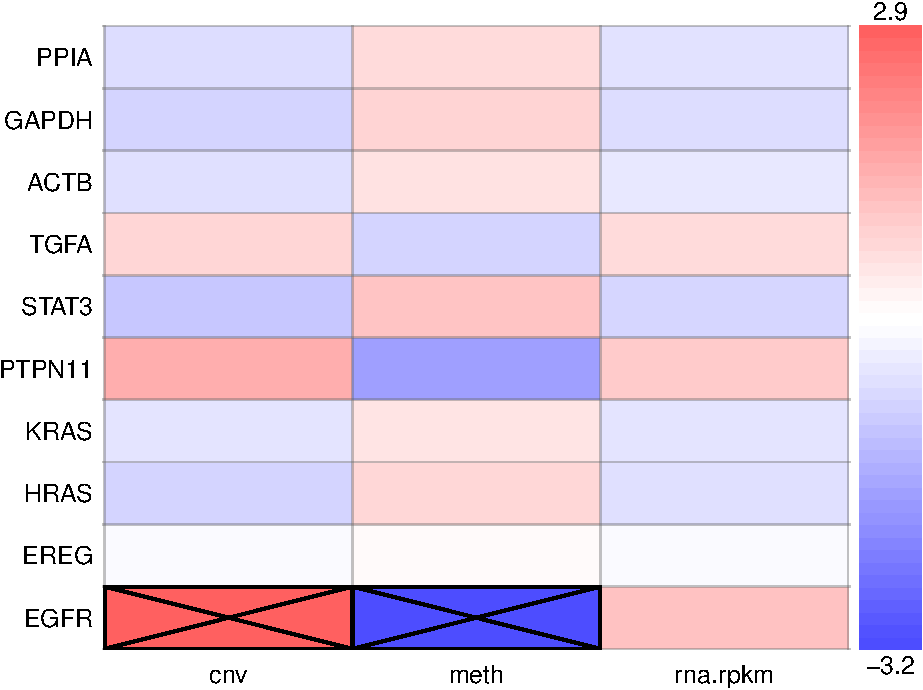
\includegraphics[width=0.45\linewidth]{chen-chang-chen-tzeng-chang_files/figure-latex/omicsplot-1} 

}

\caption[The image plot of the values for t-statistics of matrix covariate in the omics data]{The image plot of the values for t-statistics of matrix covariate in the omics data.  The effective pixels identified by the tensor regression model are marked out by the $\boxtimes$ symbol.}\label{fig:omicsplot}
\end{figure}
\end{Schunk}

\hypertarget{example-2-logistic-tensor-regression-and-classification-using-mnist-dataset}{%
\subsection{Example 2: Logistic tensor regression and classification
using MNIST
dataset}\label{example-2-logistic-tensor-regression-and-classification-using-mnist-dataset}}

MNIST is a well-known benchmark database for image recognition in
machine learning. It consists of over 60,000 training images and 10,000
testing images. For R users, one can obtain the image data from the
\CRANpkg{dslabs} package \citep{rafael2019dslabs}. For the purpose of
demonstration, we reduce the size of MNIST image data by a max-pooling
step with \(2 \times 2\) block, as shown in the images on the left and
in the middle of Figure \ref{fig:mnistpreproc}. The original
\(28 \times 28\) images are thus pixelated into \(14 \times 14\)
max-pooled images. Because pixels at the edges and the corners of the
max-pooled images take no information across almost all images, we
removed those pixels and ended up with \(P\times Q = 10 \times 10\)
sub-images as illustrated in the image on the right of Figure
\ref{fig:mnistpreproc}. The mean image of the pre-processed training set
for each label in the MNIST database is shown in Figure
\ref{fig:mnistmean}. These pre-processed images of \(10 \times 10\)
pixels are included in the package \CRANpkg{TensorTest2D} and can be
imported using the following commands:

\begin{Schunk}
\begin{figure}

{\centering 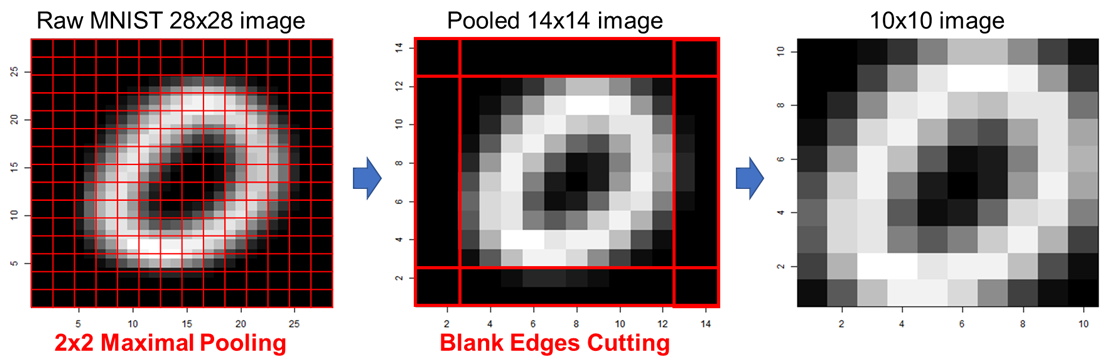
\includegraphics[width=0.95\linewidth]{chen-chang-chen-tzeng-chang_files/figure-latex/mnist_preproc} 

}

\caption[Data pre-processing for the MNIST dataset]{Data pre-processing for the MNIST dataset. First, the left subfigure shows the max-pooling step for reducing the image size. Next, the center subfigure shows the edge-cutting step for removing the noninformative pixels. Finally, the right subfigure shows the data pre-process result.}\label{fig:mnistpreproc}
\end{figure}
\end{Schunk}

\begin{Schunk}
\begin{figure}

{\centering 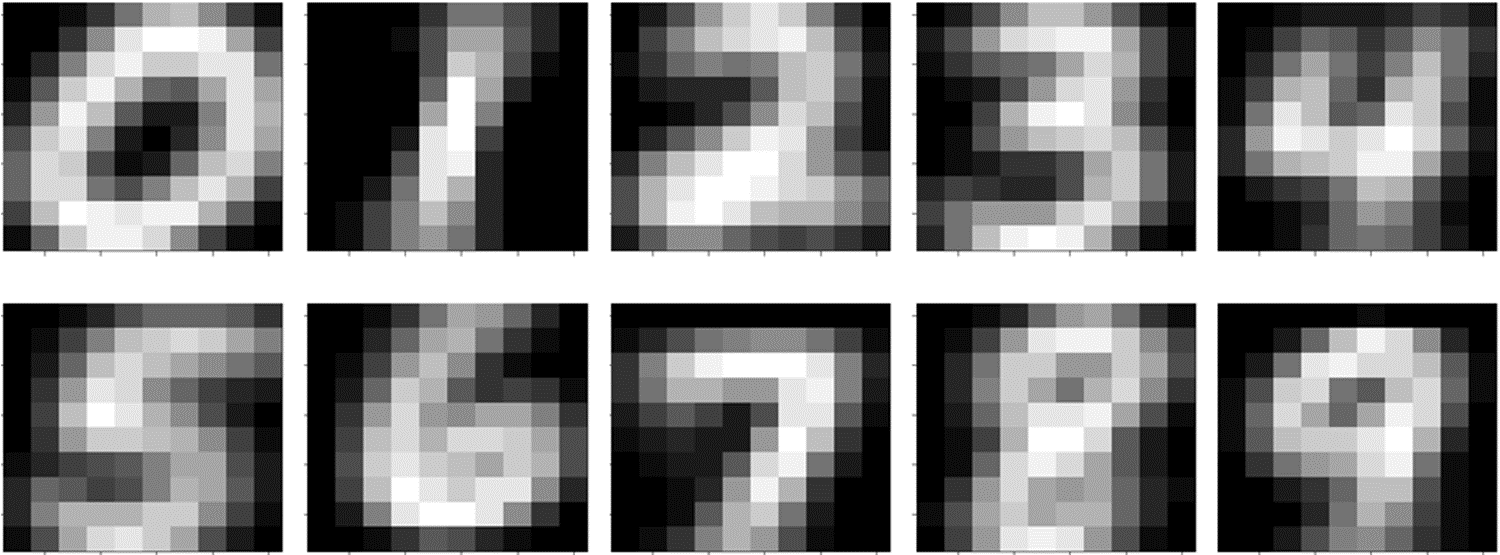
\includegraphics[width=0.95\linewidth]{chen-chang-chen-tzeng-chang_files/figure-latex/mnist_preproc_out} 

}

\caption[The mean plots of pre-processed images in the training dataset]{The mean plots of pre-processed images in the training dataset. The value at each pixel of the mean plot is the average grayscale value over the pre-processed images in the training dataset.}\label{fig:mnistmean}
\end{figure}
\end{Schunk}

\begin{Schunk}
\begin{Sinput}
library(TensorTest2D)
data(mnist_mp2c2)
mnist_train <- mnist_mp2c2$train
mnist_test <- mnist_mp2c2$test
\end{Sinput}
\end{Schunk}

The aim of this data analysis is to recognize the digit for a given
handwritten image using logistic regression. Here, we choose images of
`2' and `5' for demonstration. Let \(Y_i = 1\) if the \(i\)th image
represents the digit `5', and \(Y_i = 0\) if the \(i\)th image
represents a `2'. The predictor matrix \(X_i\) here is a
\(10 \times 10\) matrix with its entries the pixel values of the
handwritten image in grayscale. In the following, we first describe the
data processing steps and provide the code being used to obtain our
training data in the analysis. Our training data, \texttt{train\_X}, is
a \(P \times Q \times n = 10 \times 10 \times 2000\) array, which
contains subsets of 1,000 images of the digit `2' and 1,000 images of
the digit `5' randomly chosen from the MNIST training set
\texttt{mnist\_train}. In this MNIST example, some pixels in the corners
and on the edges take on the value zero across all handwritten images,
which yields singularity when the alternating maximum likelihood
algorithm is applied to the training data. To solve this problem, we can
simply drop only those zero-valued pixels. However, doing so breaks the
matrix form and hence low-rank model is no longer valid. Alternatively,
we add independent standard normal noise to the images in our training
data set that results in no significant harm to the prediction power,
because the signal-noise ratio is high and the training set sample size
is sufficiently large. Hereafter, we call images with random error the
contaminated images.

\begin{Schunk}
\begin{Sinput}
library(abind)
# Draw image data of labels 2 and 5
x0_all <- mnist_train$image[,,which(mnist_train$label == 2)]
x1_all <- mnist_train$image[,,which(mnist_train$label == 5)]
# Random sampling from MNIST training set for each label
nSampleEach <- 1000
n0 <- dim(x0_all)[3]; n1 <- dim(x1_all)[3]
set.seed(2021)
s0 <- sample(1:n0, nSampleEach, replace = FALSE)  
s1 <- sample(1:n1, nSampleEach, replace = FALSE)  
# Normalizing image values into [-0.5, 0.5]
x0 <- x0_all[,,s0]/255 - 0.5
x1 <- x1_all[,,s1]/255 - 0.5
# Combine training data
train_X <- abind(x0, x1, along = 3)
# Add negligible noise for the images 
# (so no constant zero values in one pixel over all covariate matrices)
set.seed(2021) # Set seed for reproducibility
train_n <- array((rnorm(prod(dim(train_X)), 0, 0.1)), dim(train_X))
train_Xn <- train_X + train_n # Contaminated images
# Define Y = 0 for label 2, and Y = 1 for label 5
train_y <- c(rep(0, dim(x0)[3]), rep(1, dim(x1)[3]))
\end{Sinput}
\end{Schunk}

In the package \CRANpkg{TensorTest2D}, the function
\texttt{tensorReg2D()} is also used for fitting the logistic tensor
regression model to data: \[
\log{\frac{Pr(Y_i = 1\mid\mathbf{X}_i)}{Pr(Y_i = 0\mid\mathbf{X}_i)}} = \beta +  \mathbf{X}_i \circ \mathbf{B}
\] Thus, a prediction for the digit presented in image \(\mathbf{X}_i\)
is \[
  \hat Y_i = \underset{k \in \{0,1\}}{\arg\max}\,{Pr(Y_i = k\mid\mathbf{X}_i)} = I\{Pr(Y_i = 1\mid\mathbf{X}_i) > 0.5\},
\] where \(I\{E\} = 1\), if \(E\) is true, and \(I\{E\} = 0\),
otherwise. To analyze the sampled data set, first, we feed the response
variable, \texttt{train\_y}, and the contaminated images,
\texttt{train\_Xn}, as inputs for model training. There is no auxiliary
information available to further stratify the \(y_i\)'s, we specify a
constant vector \texttt{W\ =\ matrix(1,\ length(train\_y),\ 1)} of
length \(n\), and if a rank \(R = 4\) model is needed, we set
\texttt{n\_R\ =\ 4}. (In fact, the rank-4 model is the best model in
this logistic tensor regression.)

\begin{Schunk}
\begin{Sinput}
# Train the logistic tensor regression model
lgMdl <- tensorReg2D(y = train_y, X = train_Xn, 
                      W = matrix(1, length(train_y), 1),
                      n_R = 4, family = "binomial", 
                      opt = 1, max_ite = 100, tol = 10^(-7) )
# Print model summary (not run)
#summary(lgMdl)
# Print the p-values of the estimates
cat("FDR-adjusted p-values of B_pq:\n")
\end{Sinput}
\begin{Soutput}
#> FDR-adjusted p-values of B_pq:
\end{Soutput}
\begin{Sinput}
round(matrix(p.adjust(as.vector(lgMdl$B_PV), method = "fdr"), 10, 10), 3)
\end{Sinput}
\begin{Soutput}
#>        [,1]  [,2]  [,3]  [,4]  [,5]  [,6]  [,7]  [,8]  [,9] [,10]
#>  [1,] 0.263 0.830 0.114 0.243 0.019 0.480 0.595 0.629 0.491 0.830
#>  [2,] 0.558 0.552 0.098 0.491 0.263 0.948 0.137 0.816 0.491 0.953
#>  [3,] 0.923 0.927 0.029 0.012 0.999 0.017 0.204 0.050 0.471 0.008
#>  [4,] 0.648 0.541 0.004 0.019 0.029 0.204 0.004 0.655 0.541 0.156
#>  [5,] 0.293 0.491 0.055 0.004 0.381 0.004 0.101 0.024 0.081 0.006
#>  [6,] 0.110 0.491 0.954 0.491 0.648 0.948 0.954 0.865 0.491 0.825
#>  [7,] 0.023 0.652 0.889 0.019 0.489 0.491 0.110 0.188 0.042 0.029
#>  [8,] 0.137 0.706 0.830 0.491 0.244 0.145 0.491 0.491 0.889 0.889
#>  [9,] 0.655 0.034 0.655 0.977 0.083 0.114 0.019 0.629 0.706 0.471
#> [10,] 0.137 0.055 0.491 0.764 0.491 0.602 0.019 0.471 0.454 0.025
\end{Soutput}
\end{Schunk}

For binary classification problems, we can apply the function
\texttt{plot()} of our package \CRANpkg{TensorTest2D} in two ways.
Similar to that Figure \ref{fig:omicsplot}, we can make a plot first for
the values of t-statistics for the pixels by using the \texttt{plot()}
function as shown below this paragraph. Here, we adjust the \(p\)-values
according to the approach in \cite{benjamini1995controlling} by setting
the parameter \texttt{method\ =\ "fdr"}. The resulting plot is shown in
Figure \ref{fig:mnisttval}, and most of the effective pixels can be
found on the left half side of the plot.

\begin{Schunk}
\begin{Sinput}
plot(x = lgMdl, method = "fdr", alpha = 0.05, type = "tval", 
     showlabels = TRUE, plot.legend = TRUE) 
\end{Sinput}
\begin{figure}

{\centering 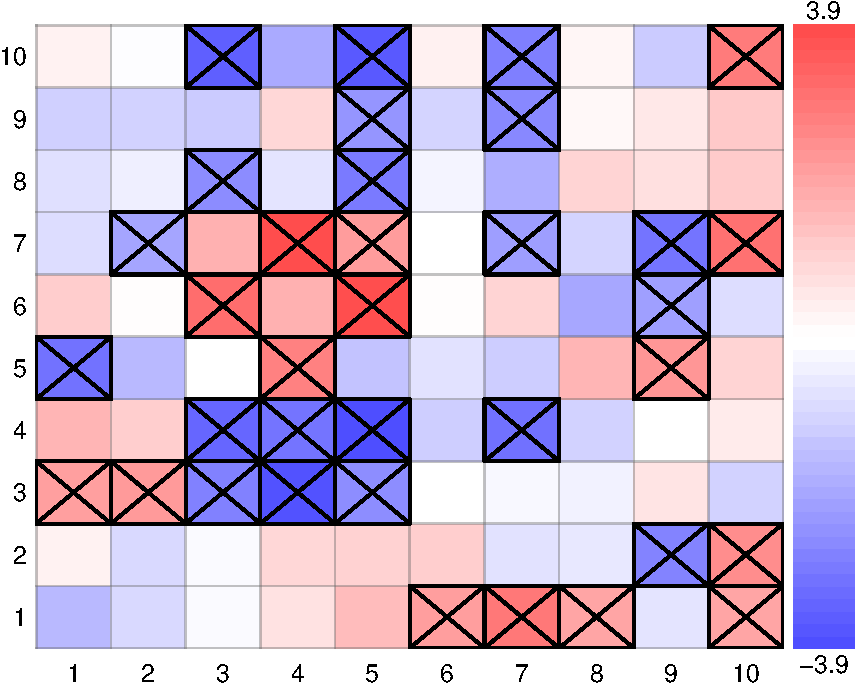
\includegraphics[width=0.45\linewidth]{chen-chang-chen-tzeng-chang_files/figure-latex/mnisttval-1} 

}

\caption[The image plot of the values for t-statistics of matrix covariate in the handwritten label data]{The image plot of the values for t-statistics of matrix covariate in the handwritten label data.  The effective pixels identified by the logistic tensor regression model are marked out by the $\boxtimes$ marks.}\label{fig:mnisttval}
\end{figure}
\end{Schunk}

To understand which areas of an image that contribute the most
information to classify between labels 2 and 5, we also add a meaningful
background image by specifying an argument to the parameter
\texttt{background} for the function \texttt{plot()}. In this example,
we show separately the mean image of label 2 and the mean image of label
5 as the background image by assigning the value \texttt{xm0} or
\texttt{xm1} to the parameter \texttt{background}. To adjust the visual
style of the background image, one can assign the value
\texttt{gray(0,\ 1,\ 0.05)} to the parameter \texttt{col} to create a
grayscale colour map for contrast. Please refer to
\texttt{help("image")} for more detail on the options available when
creating a plot. Our resulting plots are shown in Figure
\ref{fig:mnistplot}. On top of both images, there are marks for the
important pixels with red and blue frames. A red rectangle indicates
that the corresponding estimate in \(\hat{\mathbf B}\) has a significant
positive coefficient and a blue one highlights a significant negative
coefficient. In our example, important pixels are found to locate
majorly at the curvy parts of 2 and 5.

\begin{Schunk}
\begin{Sinput}
xm0 <- xm1 <- matrix(0, dim(train_X)[1], dim(train_X)[2])
# Background image: mean image of label 2
for (k in 1:dim(x0)[3]) {
  xm0 <- xm0 + (1/nSampleEach)*x0[,,k]
}
# Background image: mean image of label 5
for (k in 1:dim(x1)[3]) {
  xm1 <- xm1 + (1/nSampleEach)*x1[,,k]
}
# Draw for visualizing effective pixels for both background images 
par(mfrow = c(1, 2), mar = c(1, 1, 1, 1))
plot(x = lgMdl, method = "fdr", alpha = 0.05, background = xm0, 
     showlabels = FALSE, plot.legend = FALSE, col = gray(seq(0, 1, 0.05)))
plot(x = lgMdl, method = "fdr", alpha = 0.05, background = xm1, 
     showlabels = FALSE, plot.legend = FALSE, col = gray(seq(0, 1, 0.05)))
\end{Sinput}
\begin{figure}

{\centering 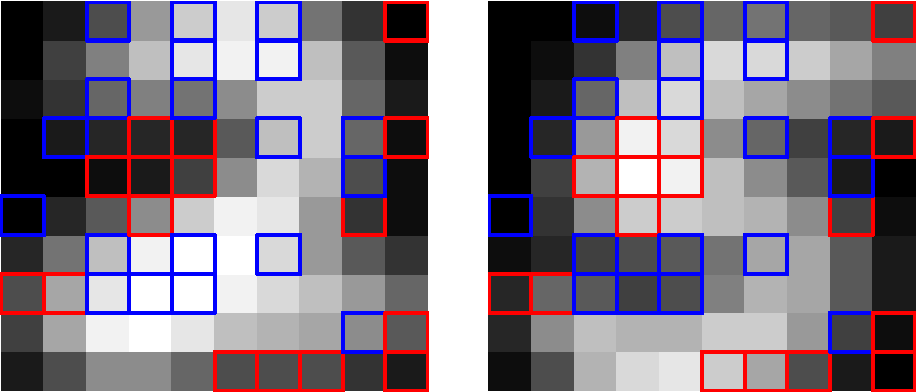
\includegraphics[width=0.95\linewidth]{chen-chang-chen-tzeng-chang_files/figure-latex/mnistplot-1} 

}

\caption[Effective pixels identified by the logistic tensor rgression model]{Effective pixels identified by the logistic tensor rgression model. The important pixels to discriminate between labels 2 and 5 are marked by red and blue frames, which indicate positive and negative coefficients, respectively.}\label{fig:mnistplot}
\end{figure}
\end{Schunk}

We use the function \texttt{predict()} to predict the label for the new
images in the testing data set. The input data must be a 3-dimensional
array of size \(P \times Q \times n^*\), where \(n^*\) is the number of
testing images. We note here that, one need to reshape the
\(P \times Q\) matrix object into the 3-dimensional array by the R
command \texttt{array(x,\ c(P,\ Q,\ 1))}. The function
\texttt{predict()} returns the predictions in two ways. By setting the
option \texttt{type\ =\ "link"}, it returns the values of the linear
predictors; and by setting \texttt{type\ =\ "response"}, it returns the
expected values of response variable. For example, for our logistic
regression model, the predictions are log-odds (odds ratios on
logarithmic scale) if \texttt{type\ =\ "link"} is chosen, or they are
the predicted probabilities of \(Y = 1\) if \texttt{type\ =\ "response"}
is chosen.

\begin{Schunk}
\begin{Sinput}
# Normalize image values of the testing data into [-0.5, 0.5]
tx0 <- mnist_test$image[,,which(mnist_test$label == 2)]/255 - 0.5
tx1 <- mnist_test$image[,,which(mnist_test$label == 5)]/255 - 0.5
# Combine testing data and assign the vector of the true responses
test_X <- abind(tx0, tx1, along = 3)
test_y <- c(rep(0, dim(tx0)[3]), rep(1, dim(tx1)[3]))
# Print some predictions with different settings of type
pred_link <- predict(lgMdl, test_X, type = "link")
pred_prob <- predict(lgMdl, test_X, type = "response")
head(round(pred_link, digits = 2))
\end{Sinput}
\begin{Soutput}
#>        [,1]
#> [1,]  -3.38
#> [2,] -16.24
#> [3,]  -4.93
#> [4,]  -5.38
#> [5,]  -9.94
#> [6,]  -6.41
\end{Soutput}
\begin{Sinput}
head(round(pred_prob, digits = 4))
\end{Sinput}
\begin{Soutput}
#>        [,1]
#> [1,] 0.0331
#> [2,] 0.0000
#> [3,] 0.0072
#> [4,] 0.0046
#> [5,] 0.0000
#> [6,] 0.0016
\end{Soutput}
\begin{Sinput}
# Compute the prediction accuracy for the testing data
pred_test_y <- (pred_prob > .5)
cat(
  sprintf("Accuracy = %2.2f%%", 
          100*sum(pred_test_y == test_y)/length(test_y)))
\end{Sinput}
\begin{Soutput}
#> Accuracy = 96.10%
\end{Soutput}
\end{Schunk}

In addition, we provide a visualization tool that works with other
methods in variable selection for 2D images. For example, the penalized
regression via lasso \citep{tibshirani1996regression} is one of the
popular approaches. Below are the codes that we implemented to train a
LASSO model, including the use of the function \texttt{cv.glmnet()}
\citep{friedman2010regularization}. The object \texttt{l1B} is the
\(10\times10\) array of LASSO estimates. Since LASSO tends to shrink
small coefficients to zero, we treat those image pixels with zero-valued
coefficients to be irrelevant to distinguish between images of 2 and 5.
To visualize the effective pixels identified by LASSO, our package
\CRANpkg{TensorTest2D} provides the function \texttt{draw.coef()} to
produce the marked image similar to that in Figure \ref{fig:mnistplot}.
Different from the function \texttt{plot.tsglm()}, users need to provide
an input as the markers for effective pixels. The markers in our example
here are the LASSO estimates, and by specifying \texttt{marks\ =\ l1B},
the pixels with non-zero coefficients are then marked. In addition, by
specifying \texttt{markstyle\ =\ "bi-dir"}, as shown in Figure
\ref{fig:mnistlasso}, the pixels marked out with red rectangles
correspond to those of positive LASSO estimates, and the pixels with
blue rectangles are those of negative LASSO estimates.

\begin{Schunk}
\begin{Sinput}
library(glmnet)
# Vectorize the hand-written images
xv <- t(sapply(1:dim(train_X)[3], function(k) as.vector(train_X[,,k])))
# Train the LASSO model using cross-validation
set.seed(2021) # Set seed for reproducibility
l1Mdl <- cv.glmnet(xv, train_y, family = "binomial", alpha = 1, standardize = FALSE)
# Draw the LASSO coefficients from the best model
l1B <- matrix(l1Mdl$glmnet.fit$beta[,which.min(l1Mdl$cvm)], 10, 10)
# The LASSO estimates
print(round(l1B, digits = 3))
\end{Sinput}
\begin{Soutput}
#>         [,1]   [,2]   [,3]   [,4]   [,5]   [,6]   [,7]   [,8]   [,9]  [,10]
#>  [1,] -0.247  0.000  0.253  0.000 -0.409  0.000  0.000  0.000  0.000  0.000
#>  [2,] -0.559  0.000  0.000  0.000 -0.200  0.000  0.000  0.000 -0.691  0.000
#>  [3,]  0.000  0.000 -0.248 -0.513  0.000  1.287  0.000  0.000  0.000 -0.914
#>  [4,]  0.000  0.000 -1.526 -1.805  0.734  1.237  1.804  0.000  0.000 -0.254
#>  [5,]  0.142  0.000 -0.593 -0.795  0.000  1.280  0.929  0.000 -0.699 -0.738
#>  [6,]  1.625 -0.251  0.000 -1.429 -0.527  0.000  0.000  0.000  0.000 -0.592
#>  [7,]  0.592 -0.136 -0.668 -0.554  0.000  0.000  0.000 -0.406 -0.397 -0.285
#>  [8,]  0.074 -0.204  0.000 -0.757  0.265 -0.211 -1.082  0.000  0.000  0.000
#>  [9,]  0.000 -0.574  0.000  0.000  0.360 -1.558  0.000  0.000  0.638  0.000
#> [10,]  0.000  0.000 -0.628 -0.144  0.000  0.000  0.479  1.340  0.303  0.845
\end{Soutput}
\begin{Sinput}
# Draw for visualizing effective pixels identified by LASSO for both background images 
par(mfrow = c(1, 2), mar = c(1, 1, 1, 1))
draw.coef(img = xm0, marks = l1B, markstyle = "bi-dir", showlabels = FALSE, 
          plot.legend = FALSE, grids = FALSE, col = gray(seq(0, 1, 0.05)))
draw.coef(img = xm1, marks = l1B, markstyle = "bi-dir", showlabels = FALSE, 
          plot.legend = FALSE, grids = FALSE, col = gray(seq(0, 1, 0.05)))
\end{Sinput}
\begin{figure}

{\centering 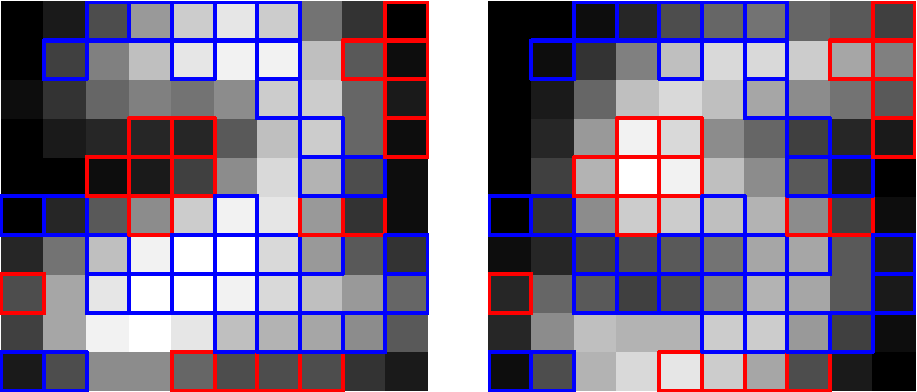
\includegraphics[width=0.95\linewidth]{chen-chang-chen-tzeng-chang_files/figure-latex/mnistlasso-1} 

}

\caption[Effective pixels identified by the LASSO model]{Effective pixels identified by the LASSO model. The important pixels to discriminate between labels 2 and 5 are marked by red and blue frames, which indicate positive and negative coefficients, respectively.}\label{fig:mnistlasso}
\end{figure}
\end{Schunk}

\hypertarget{summary}{%
\section{Summary}\label{summary}}

Issues in estimation and test of hypothesis that emerged from fitting
regression models with predictor variables that has a matrix form are of
our major interest. Low-rank modelling can be applied to improve the
efficiency of estimation. In this line, we developed the R package
\CRANpkg{TensorTest2D} to conduct tensor regression analysis within the
framework of generalized linear models. In addition to model estimation
and hypothesis testing, this package also includes a visualization tool
that can be used to indicate the positions of effective or significant
pixels when the tensor predictor is of image data type.

\bibliography{chen-chang-chen-tzeng-chang}


\address{%
Ping-Yang Chen\\
Chimes AI\\%
12F., No.~201-8, Dunhua N. Rd., Songshan Dist.,\\ Taipei City 105076,
Taiwan\\
%
%
%
\href{mailto:pychen@chimes.ai}{\nolinkurl{pychen@chimes.ai}}%
}

\address{%
Hsing-Ming Chang\\
Department of Statistics and Institute of Data Science, National Cheng
Kung University\\%
1 University Road,\\ Tainan 70101, Taiwan\\
%
%
%
\href{mailto:nckuhmchang@ncku.edu.tw}{\nolinkurl{nckuhmchang@ncku.edu.tw}}%
}

\address{%
Yu-Ting Chen\\
Department of Statistics, Purdue University\\%
250 N. University St, West Lafayette,\\ IN 47907, United States of
America\\
%
%
%
\href{mailto:l501l501l@gmail.com}{\nolinkurl{l501l501l@gmail.com}}%
}

\address{%
Jung-Ying Tzeng\\
Department of Statistics and Bioinformatics Research Center, North
Carolina State University\\%
North Carolina State University\\ Raleigh NC, 27695, United States of
America\\
%
%
%
\href{mailto:jytzeng@ncsu.edu}{\nolinkurl{jytzeng@ncsu.edu}}%
}

\address{%
Sheng-Mao Chang\\
Department of Statistics, National Taipei University\\%
No.~151, University Rd., Sanxia Dist.,\\ New Taipei City 237303,
Taiwan\\ Corresponding Author\\
%
%
%
\href{mailto:smchang110@gm.ntpu.edu.tw}{\nolinkurl{smchang110@gm.ntpu.edu.tw}}%
}
